\tikzstyle{rblock} = [rectangle, draw, text width=15em, text centered, inner sep=0pt, minimum height=2em, rounded corners]
\tikzstyle{line} = [draw, -latex']
\tikzstyle{arrow} = [thick,->,>=stealth]

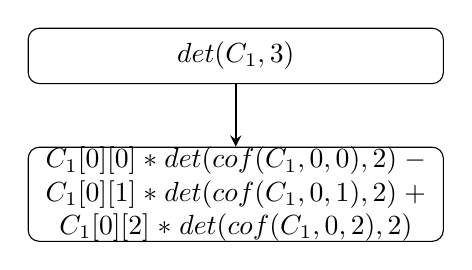
\begin{tikzpicture}[node distance = 5em, auto]
    \node (node3) [rblock] {$det(C_1, 3)$};
    \node (node4) [rblock, below of = node3] {$C_1[0][0] * det(cof(C_1, 0, 0), 2) - C_1[0][1] * det(cof(C_1, 0, 1), 2) + C_1[0][2] * det(cof(C_1, 0, 2), 2)$};
    \draw [arrow] (node3) -- (node4);
\end{tikzpicture}